Este cap\'{i}tulo describe el proceso seguido para la generaci\'{o}n del modelo de detecci\'{o}n de anomal\'{i}as de manejo. Seg\'{u}n lo repasado en el cap\'{i}tulo anterior, en el presente trabajo, se propone un m\'{e}todo de detecci\'{o}n de anomal\'{i}as de conducci\'{o}n siguiendo un enfoque semi-supervisado; sin embargo, antes de profundizar en el m\'{e}todo propuesto se debe realizar un repaso del conjunto de datos con el que se cuenta en la investigaci\'{o}n.

\section{Conjunto de datos normales y an\'{o}malos}

En el Cap\'{i}tulo 3 se describi\'{o} el proceso de captura y preparaci\'{o}n del conjunto de datos, as\'{i} como tambi\'{e}n su divisi\'{o}n en conjunto de entrenamiento/desarrollo/prueba; sin embargo cabe aclarar que aquel cap\'{i}tulo s\'{o}lo se enfoc\'{o} en el  \textbf{conjunto de datos normales}, los cuales corresponden a aquellos datos que no cuentan con una etiqueta.%; por lo que es el conjunto que se usa para entrenar el modelo que se ajusta al comportamiento normal de manejo.

\vspace{5mm} %5mm vertical space

A pesar de contar con una gran cantidad de datos normales se debe recolectar datos que correspondan a anomal\'{i}as con el objetivo de poder validar el m\'{e}todo que se propone en este proyecto. Por lo que se debi\'{o} proceder a la captura de  \textbf{datos an\'{o}malos}, el cual est\'{a} conformado seg\'{u}n el Cuadro \ref{table:conjunto_anomalias}.

\begin{table}[]
\centering
\begin{tabular}{|l|l|l|}
\hline
Tipo de anomal\'{i}a & Nro anomal\'{i}as & Nro de datos \\ \hline
Frenos en seco    & 15  & 100  \\ \hline
Giros a la derecha e izquierda a alta velocidad & 15  & 450  \\ \hline
Giros en U a alta velocidad & 100 & 300 \\ \hline
\end{tabular}
\caption{Tabla del conjunto de anomal\'{i}as.}
\label{table:conjunto_anomalias}
\end{table}

\vspace{5mm} %5mm vertical space

Como se mencion\'{o} en el anterior p\'{a}rrafo el conjunto de anomal\'{i}as fue capturado para validar el m\'{e}todo propuesto, por lo que este conjunto ser\'{a} etiquetado como positivo (con la etiqueta 1) y el conjunto de datos normales ser\'{a} etiquetado como muestras negativas (con la etiqueta 0).

\subsection{Generaci\'{o}n de series temporales}

Para la generaci\'{o}n del modelo detector de anomal\'{i}as se opt\'{o} por algoritmos de aprendizaje autom\'{a}tico enfocados en series de tiempo, dado que los datos capturados por el dispositivo m\'{o}vil, dependen del tiempo en el que fueron capturados; por lo cual el primer paso a realizar es la generaci\'{o}n de peque\~{n}as fracciones de series temporales, esto permitir\'{a} que el modelo propuesto vaya m\'{a}s all\'{a} de una simple detecci\'{o}n de anomal\'{i}as puntuales y pueda detectar anomal\'{i}as contextuales o colectivas.

\vspace{5mm} %5mm vertical space

En el Cuadro \ref{table:series-de-tiempo} se presenta los resultados de diferentes tama\~{n}os de series de tiempo, observando estos resultados en primera instancia se descarta la serie de tiempo que cuenta con uno y dos pasos; debido a que no son lo suficientemente descriptivos. En cuanto a las series de tiempo restantes no es posible definir a\'{u}n cual es la cantidad correcta de pasos, por lo cual al igual que la cantidad de componentes principales, ser\'{a} un par\'{a}metro a optimizar en los diferentes experimentos que se realizar\'{a} en las siguientes secciones. Cabe recalcar que el dominio de \'{e}sta variable estar\'{a} entre 3 a 5 pasos y el de la cantidad de componentes principales estar\'{a} entre 3 y 4.

\begin{table}[]
\centering
\begin{center}
\begin{tabular}{cl|l|l|}
\cline{3-4}
\multicolumn{1}{l}{} &   & \multicolumn{2}{c|}{\textbf{Nro de componentes}} \\ \cline{3-4} 
\multicolumn{1}{l}{} &   & \multicolumn{1}{c|}{3} & \multicolumn{1}{c|}{4} \\ \hline
\multicolumn{1}{|c|}{\multirow{5}{*}{\rotatebox{90}{\textbf{Tama\~{n}os de series de tiempo}}}} & \multicolumn{1}{c|}{1} & \adj{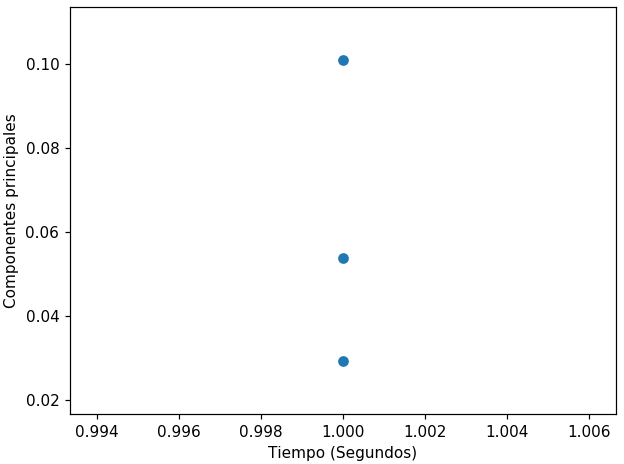
\includegraphics[width=1.85in]{imagenes/Cap4/pca3-1}} & \adj{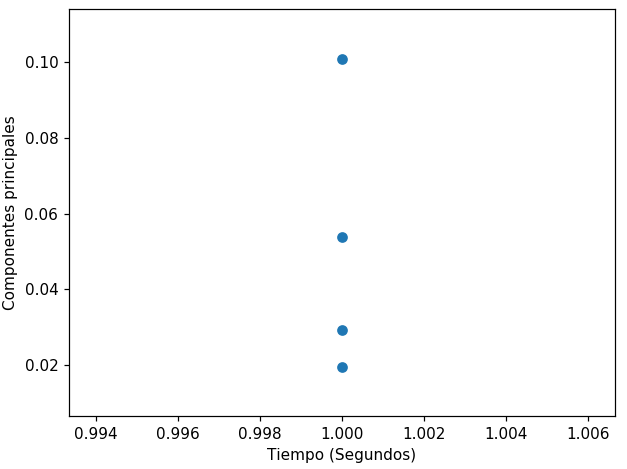
\includegraphics[width=1.85in]{imagenes/Cap4/pca4-1}}  \\ \cline{2-4} 
\multicolumn{1}{|c|}{}                                             & \multicolumn{1}{c|}{2} & \adj{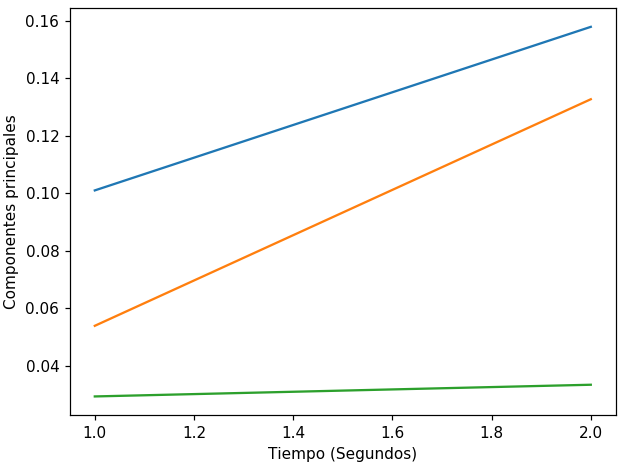
\includegraphics[width=1.85in]{imagenes/Cap4/pca3-2}}  & \adj{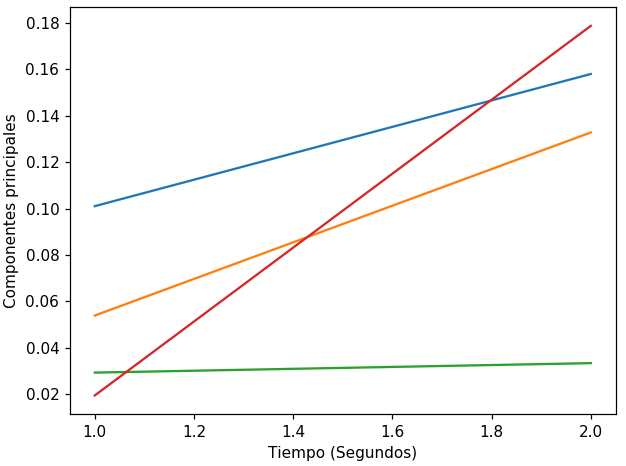
\includegraphics[width=1.85in]{imagenes/Cap4/pca4-2}} \\ \cline{2-4} 
\multicolumn{1}{|c|}{}                                             & 3 & \adj{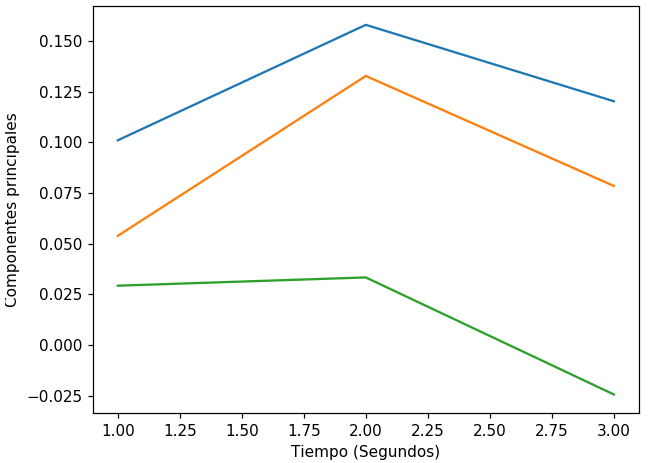
\includegraphics[width=1.85in]{imagenes/Cap4/pca3-3}} & \adj{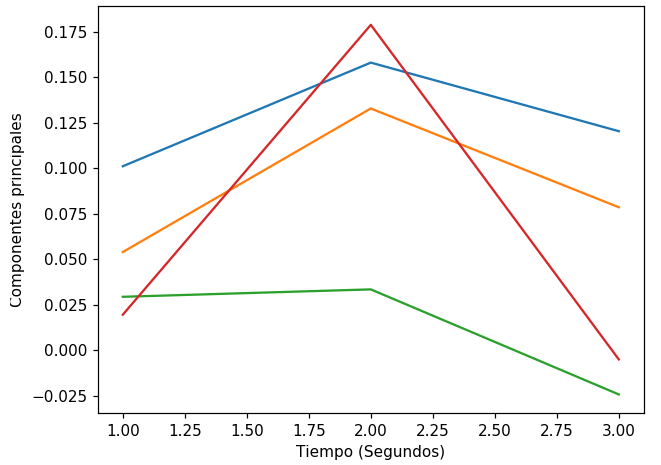
\includegraphics[width=1.85in]{imagenes/Cap4/pca4-3}} \\ \cline{2-4} 
\multicolumn{1}{|c|}{}                                             & 4 & \adj{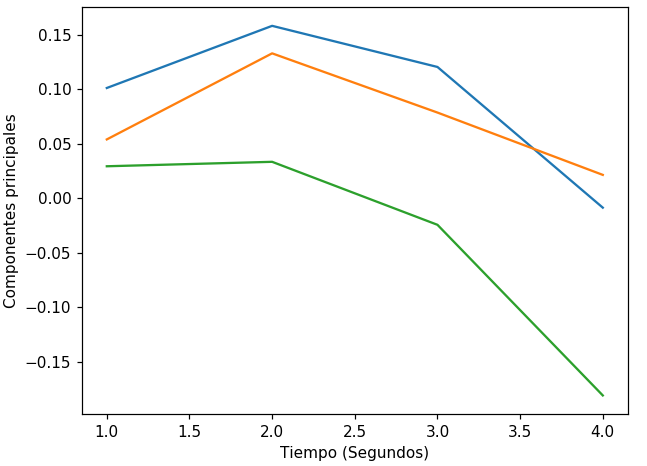
\includegraphics[width=1.85in]{imagenes/Cap4/pca3-4}} & \adj{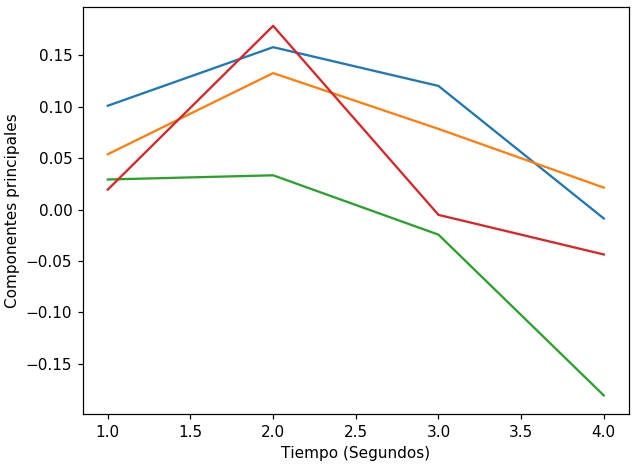
\includegraphics[width=1.85in]{imagenes/Cap4/pca4-4}} \\ \cline{2-4} 
\multicolumn{1}{|c|}{}                                             & 5 & \adj{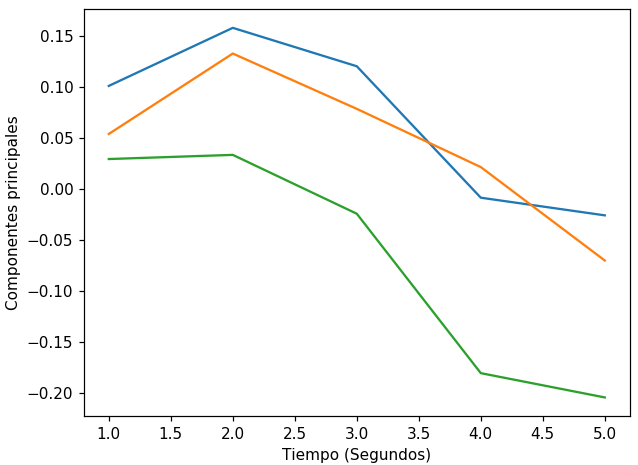
\includegraphics[width=1.85in]{imagenes/Cap4/pca3-5}} & \adj{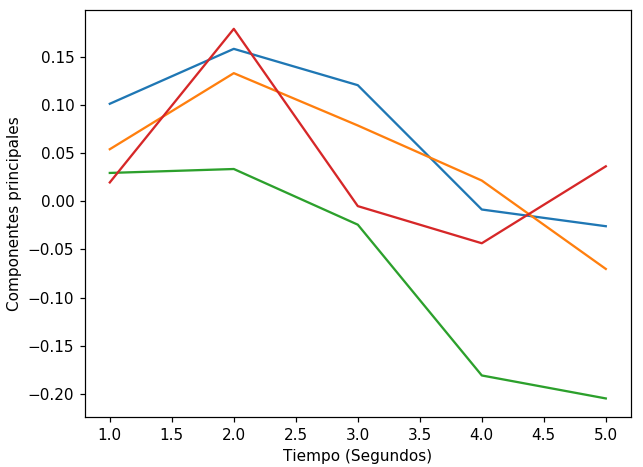
\includegraphics[width=1.85in]{imagenes/Cap4/pca4-5}} \\ \hline
\end{tabular}
\end{center}
\caption{Tabla con diferentes tama\~{n}os de series de tiempo para 3 y 4 componentes principales.}
  \label{table:series-de-tiempo}
\end{table}

\section{Modelo de detecci\'{o}n de anomal\'{i}as}

Como se mencion\'{o} previamente en la presente investigaci\'{o}n se propone un m\'{e}todo de detecci\'{o}n de anomal\'{i}as de conducci\'{o}n siguiendo un enfoque semi-supervisado, el cual consta de dos componentes: un \textbf{modelo ajustado al comportamiento normal} de manejo de un agente y un \textbf{m\'{e}todo de umbral para la detecci\'{o}n de valores at\'{i}picos}.

\vspace{5mm} %5mm vertical space

Para la presente investigaci\'{o}n se har\'{a} la comparaci\'{o}n entre 3 diferentes m\'{e}todos de detecci\'{o}n, y seg\'{u}n el rendimiento de cada uno se elegir\'{a} la mejor opci\'{o}n. En el Cuadro \ref{table:metodos_comparados} se presenta los tres diferentes m\'{e}todos que ser\'{a}n comparados y como se puede observar para todos los casos se usa un autoencoder como modelo del comportamiento normal, por lo que las siguientes secci\'{o}nes se enfocar\'{a}n en la descripci\'{o}n del entrenamiento del autoencoder, para posteriormente probar los 3 diferentes tipos de detecci\'{o}n de anomal\'{i}as.

\begin{table}[]
\centering
\begin{tabular}{|l|p{100mm}|}
\hline
\textbf{M\'{e}todo} & \textbf{Descripci\'{o}n} \\ \hline
AE\_T & M\'{e}todo de detecci\'{o}n basado en autoencoders y umbralizaci\'{o}n (Thresholding) \\ \hline
AE\_IF & M\'{e}todo de detecci\'{o}n basado en autoencoders y la aplicaci\'{o}n de Isolation Forest sobre la codificaci\'{o}n obtenida por el autoencoder  \\ \hline
AE\_OC-SVM & M\'{e}todo de detecci\'{o}n basado en autoencoders y la aplicaci\'{o}n de One-Class SVM sobre la codificaci\'{o}n obtenida por el autoencoder \\ \hline
\end{tabular}
\caption{Tabla de los m\'{e}todos comparados.}
\label{table:metodos_comparados}
\end{table}

\subsection{Modelo del comportamiento normal}

Esta etapa es una de las partes m\'{a}s importantes de \'{e}ste trabajo debido a que el rendimiendo del modelo de detecci\'{o}n de anomal\'{i}as depende en gran parte de la precisi\'{o}n de esta etapa.

\vspace{5mm} %5mm vertical space

Como se mencion\'{o} en la anterior secci\'{o}n en esta etapa se utilizar\'{a} un autoencoder como modelo ajustado al comportamiento normal de manejo. Por lo cual el autoencoder se entren\'{o} con el conjunto de datos normales, de manera que el modelo aprenda a generar s\'{o}lo las clases que se consideran normales y, con suerte, tendr\'{a} problemas para reconstruir anomal\'{i}as, debido a que estas muestras no fueron presentadas durante el entrenamiento.

\vspace{5mm} %5mm vertical space

Para ello se prob\'{o} con diferentes arquitecturas, los detalles se presentan en el Cuadro ... .



\vspace{5mm} %5mm vertical space



\vspace{5mm} %5mm vertical space